\section{Aufgabe 2} \label{ex2}
In der Aufgabe 2 wurde eine Funktion zum zeichnen eines Quadrates variabler Position und Größe (size) geschrieben. Diese kann 
dann direkt verwendet werden um komplexere Muster mit übergeordnetem Koordinatensystem zu zeichnen, wie z.B. Arcade Figuren.

\subsection{C-Code}
C-Code zur Generierung von geometrischen Figuren. Es wurden Quadrate und darauf aufbauend eine Space-Invaders 
Figure kreiert. Zusätzlich können über die Hardware-Switches drei verschiedene Modi umgeschaltet werden:\\
BTN0: Toggle Augenfarbe zwischen rot und blau\\
BTN1: Hintergrundfarbe umschalten zwsichen blau/weiss\\

\begin{verbatim}
/* ------------------------------------------------
 * | UART TYPE   BAUD RATE                      |
 * ------------------------------------------------
 *   uartns550   9600
 *   uartlite    Configurable only in HW design
 *   ps7_uart    115200 (configured by bootrom/bsp)
 */
#include  <stdio.h>
#include  <stdlib.h>
#include  <time.h>

#include "platform.h"
//  Include  Files
#include "xparameters.h"
#include "xgpio.h"
#include "xstatus.h"
#include "xil_printf.h"
#include "lab3_a1_vga_v2.h"

//  Definitions
#define BASE_ADDR 0x43C00000
#define  SW_DEVICE_ID  XPAR_AXI_GPIO_0_DEVICE_ID

#define  LED_DELAY  10000000
#define  LED_CHANNEL 1
#define  printf  xil_printf

XGpio  SWInst; // LEDInst
static int sw_value ;

#define BTN0 1
#define BTN1 2
#define BTN2 4
#define BTN3 8
#define BTN4 16
#define BTN5 32
#define BTN6 64
#define BTN7 128

#define EYE 2
#define BODY 46

typedef enum _color {
	eW = 0,
	eR  = 1,
	eG  = 2,
	eB  = 3
} ecolor;

typedef struct _coord {
	int x;
	int y;
} coord;

// Arcade Figur
uint eyex[EYE] = {3,7};
uint eyey[EYE] = {3,3};
uint spx[BODY] = {2,8,3,7, 2,3,4,5,6,7,8, 1,2,4,5,6,8,9, 
                     0,1,2,3,4,5,6,7,8,9,10, 0,2,3,4,5,6,7,8,10, 0,2,8,10, 3,4,6,7};
uint spy[BODY] = {0,0,1,1, 2,2,2,2,2,2,2, 3,3,3,3,3,3,3, 
                    4,4,4,4,4,4,4,4,4,4, 4, 5,5,5,5,5,5,5,5, 5, 6,6,6, 6, 7,7,7,7};

void paintsquare(uint x, uint y, uint size, ecolor color) {
	if (x < 0 || x > 630)
		return;
	if (y < 0 || y > 470)
		return;
		
	uint i,j;
	for (i = x; i < x+size; ++i)
		for (j = y; j < y+size; ++j)
			LAB3_A1_VGA_V2_mWriteReg((u32)BASE_ADDR, 0, (i << 11 | j << 2 | color));
} 

void resetbg (ecolor color) {
	int i,j;
	for (i = 0; i < 680; ++i)
		for (j = 0; j < 480; ++j)
			LAB3_A1_VGA_V2_mWriteReg((u32)BASE_ADDR, 0, (i << 11 | j << 2 | color));
}

int  main()
{
	double DELAY = 10000000,z;
	init_platform ();
	int status ;

	// Initialise Push Buttons
	status = XGpio_Initialize (&SWInst , SW_DEVICE_ID );
	if ( status != XST_SUCCESS )
		return XST_FAILURE ;
	XGpio_SetDataDirection (&SWInst,1,0xFF);

	print("Hello world\n\r");

	//SWReadExample ();
	uint i,j;
	coord pos = {100,100};
	coord pos_new = {100,100};
	
	uint write_new = 1;
	uint delete = 0;
	uint background_repaint = 0;
	ecolor bgcolor = eW;

	uint size = 10;
	ecolor color = eR;
	uint btn0_on = 0, btn1_on = 0;

	resetbg(bgcolor);

	while (1) {

		sw_value = XGpio_DiscreteRead (&SWInst , 1);
		/* toggle eye color */
		if (btn0_on != (sw_value & BTN0) ) {
			write_new = 1;
			btn0_on = sw_value & BTN0;

			if (btn0_on == BTN0)
				color = eB;
			else
				color = eR;
		}

		/* toggle bg color */
		if (btn1_on != (sw_value & BTN1) ) {
			write_new = 1;
			btn1_on = sw_value & BTN1;

			xil_printf ("Switch 2: %x\n\r",(sw_value & BTN2));
			if (btn1_on == BTN1) {
				xil_printf ("Switch 2 = 1: %d\n\r",1);
				bgcolor = eB;
				resetbg(bgcolor);
			}
			else {
				bgcolor = eW;
				resetbg(bgcolor);
			}
		}

		if (write_new) {
			  // do we need wait statements to not write too fast to the FPGA
			  for (i = 0; i < EYE; ++i)
			  	paintsquare(pos.x + size*eyex[i], pos.y + size*eyey[i], size, color);
			  for (i = 0; i < BODY; ++i)
			  	paintsquare(pos.x + size*spx[i], pos.y + size*spy[i], size, eG);
			
			  write_new--;
		}
		
		sleep(1);

	}; // while

	cleanup_platform ();
	return  0;
}
\end{verbatim}

\begin{minipage}{\textwidth}
    \begin{center}        
        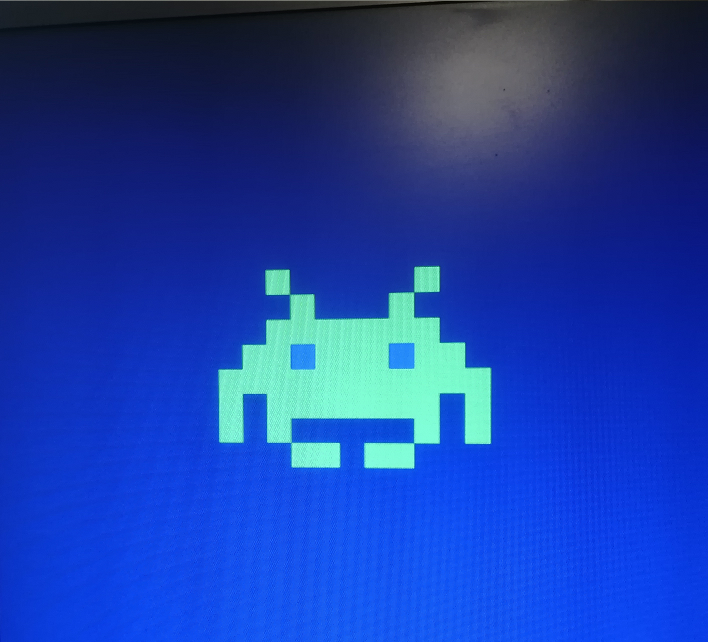
\includegraphics[scale=0.5]{img/blue.png} 
    \end{center}
\end{minipage}
\begin{center}
Arcade-SpaceInvader mit blauem Hintergrund
\end{center}





